\PassOptionsToPackage{unicode=true}{hyperref} % options for packages loaded elsewhere
\PassOptionsToPackage{hyphens}{url}
%
\documentclass[]{article}
\renewcommand{\figurename}{Hình}
\renewcommand{\tablename}{Bảng}
\usepackage{lmodern}
\usepackage{amssymb,amsmath}
\usepackage{ifxetex,ifluatex}
\usepackage{fixltx2e} % provides \textsubscript
\ifnum 0\ifxetex 1\fi\ifluatex 1\fi=0 % if pdftex
  \usepackage[T1]{fontenc}
  \usepackage[utf8]{inputenc}
  \usepackage{textcomp} % provides euro and other symbols
\else % if luatex or xelatex
  \usepackage{unicode-math}
  \defaultfontfeatures{Ligatures=TeX,Scale=MatchLowercase}
\fi
% use upquote if available, for straight quotes in verbatim environments
\IfFileExists{upquote.sty}{\usepackage{upquote}}{}
% use microtype if available
\IfFileExists{microtype.sty}{%
\usepackage[]{microtype}
\UseMicrotypeSet[protrusion]{basicmath} % disable protrusion for tt fonts
}{}
\IfFileExists{parskip.sty}{%
\usepackage{parskip}
}{% else
\setlength{\parindent}{0pt}
\setlength{\parskip}{6pt plus 2pt minus 1pt}
}

\usepackage{color}
\usepackage{fancyvrb}
\newcommand{\VerbBar}{|}
\newcommand{\VERB}{\Verb[commandchars=\\\{\}]}
\DefineVerbatimEnvironment{Highlighting}{Verbatim}{commandchars=\\\{\},breaklines=true,breakanywhere=true,fontsize=\small,frame=single,framesep=2mm,rulecolor=\color{gray}}
% Add ',fontsize=\small' for more characters per line
\newenvironment{Shaded}{}{}
\newcommand{\AlertTok}[1]{\textcolor[rgb]{1.00,0.00,0.00}{\textbf{#1}}}
\newcommand{\AnnotationTok}[1]{\textcolor[rgb]{0.38,0.63,0.69}{\textbf{\textit{#1}}}}
\newcommand{\AttributeTok}[1]{\textcolor[rgb]{0.49,0.56,0.16}{#1}}
\newcommand{\BaseNTok}[1]{\textcolor[rgb]{0.25,0.63,0.44}{#1}}
\newcommand{\BuiltInTok}[1]{#1}
\newcommand{\CharTok}[1]{\textcolor[rgb]{0.25,0.44,0.63}{#1}}
\newcommand{\CommentTok}[1]{\textcolor[rgb]{0.38,0.63,0.69}{\textit{#1}}}
\newcommand{\CommentVarTok}[1]{\textcolor[rgb]{0.38,0.63,0.69}{\textbf{\textit{#1}}}}
\newcommand{\ConstantTok}[1]{\textcolor[rgb]{0.53,0.00,0.00}{#1}}
\newcommand{\ControlFlowTok}[1]{\textcolor[rgb]{0.00,0.44,0.13}{\textbf{#1}}}
\newcommand{\DataTypeTok}[1]{\textcolor[rgb]{0.56,0.13,0.00}{#1}}
\newcommand{\DecValTok}[1]{\textcolor[rgb]{0.25,0.63,0.44}{#1}}
\newcommand{\DocumentationTok}[1]{\textcolor[rgb]{0.73,0.13,0.13}{\textit{#1}}}
\newcommand{\ErrorTok}[1]{\textcolor[rgb]{1.00,0.00,0.00}{\textbf{#1}}}
\newcommand{\ExtensionTok}[1]{#1}
\newcommand{\FloatTok}[1]{\textcolor[rgb]{0.25,0.63,0.44}{#1}}
\newcommand{\FunctionTok}[1]{\textcolor[rgb]{0.02,0.16,0.49}{#1}}
\newcommand{\ImportTok}[1]{#1}
\newcommand{\InformationTok}[1]{\textcolor[rgb]{0.38,0.63,0.69}{\textbf{\textit{#1}}}}
\newcommand{\KeywordTok}[1]{\textcolor[rgb]{0.00,0.44,0.13}{\textbf{#1}}}
\newcommand{\NormalTok}[1]{#1}
\newcommand{\OperatorTok}[1]{\textcolor[rgb]{0.40,0.40,0.40}{#1}}
\newcommand{\OtherTok}[1]{\textcolor[rgb]{0.00,0.44,0.13}{#1}}
\newcommand{\PreprocessorTok}[1]{\textcolor[rgb]{0.74,0.48,0.00}{#1}}
\newcommand{\RegionMarkerTok}[1]{#1}
\newcommand{\SpecialCharTok}[1]{\textcolor[rgb]{0.25,0.44,0.63}{#1}}
\newcommand{\SpecialStringTok}[1]{\textcolor[rgb]{0.73,0.40,0.53}{#1}}
\newcommand{\StringTok}[1]{\textcolor[rgb]{0.25,0.44,0.63}{#1}}
\newcommand{\VariableTok}[1]{\textcolor[rgb]{0.10,0.09,0.49}{#1}}
\newcommand{\VerbatimStringTok}[1]{\textcolor[rgb]{0.25,0.44,0.63}{#1}}
\newcommand{\WarningTok}[1]{\textcolor[rgb]{0.38,0.63,0.69}{\textbf{#1}}}
\usepackage{longtable,booktabs}
\IfFileExists{footnote.sty}{\usepackage{footnote}\makesavenoteenv{longtable}}{}
\usepackage{graphicx,grffile}
\makeatletter
\def\maxwidth{\ifdim\Gin@nat@width>\linewidth\linewidth\else\Gin@nat@width\fi}
\def\maxheight{\ifdim\Gin@nat@height>\textheight\textheight\else\Gin@nat@height\fi}
\makeatother
\setkeys{Gin}{width=\maxwidth,height=\maxheight,keepaspectratio}
\setlength{\emergencystretch}{3em}  % prevent overfull lines
\providecommand{\tightlist}{%
  \setlength{\itemsep}{0pt}\setlength{\parskip}{0pt}}
\setcounter{secnumdepth}{0}

\usepackage{fontspec}
\setmainfont{Times New Roman}

%-------------------------------------------------------------
% 2) LAYOUT TRANG
%-------------------------------------------------------------
\usepackage[a4paper, left=2.5cm, right=2.5cm, top=4cm, bottom=3.2cm,
            headheight=2.6cm, headsep=0.6cm, footskip=1.6cm]{geometry}

%-------------------------------------------------------------
% 3) MÀU SẮC
%-------------------------------------------------------------
\usepackage{xcolor}
\definecolor{primary}{HTML}{004AAD}   % Primary Blue
\definecolor{secondary}{HTML}{E8630A} % Secondary Orange

%-------------------------------------------------------------
% 4) HEADER / FOOTER + DIVIDER MÀU
%-------------------------------------------------------------
\usepackage{graphicx}
\usepackage{fancyhdr}
\usepackage{lastpage}

\pagestyle{fancy}
\fancyhf{}

\renewcommand{\headrulewidth}{1.2pt}
\renewcommand{\footrulewidth}{1.2pt}
\renewcommand{\headrule}{{\color{primary}\hrule height\headrulewidth}}
\renewcommand{\footrule}{{\color{primary}\hrule height\footrulewidth}}

\fancyhead[L]{\raisebox{-0.15cm}{\includegraphics[height=1.3cm]{../aiguru-logo.png}}}
\fancyhead[R]{\raisebox{-0.15cm}{\includegraphics[height=1.3cm]{../tinix-logo.png}}}

\fancyfoot[L]{\fontsize{10}{12}\selectfont By AI Guru. SĐT: 0392 121 080}
\fancyfoot[R]{\fontsize{10}{12}\selectfont Trang \thepage/\pageref{LastPage}}

% Giữ nguyên header/footer cho trang plain
\fancypagestyle{plain}{%
  \fancyhf{}
  \fancyhead[L]{\raisebox{-0.15cm}{\includegraphics[height=1.3cm]{../aiguru-logo.png}}}
  \fancyhead[R]{\raisebox{-0.15cm}{\includegraphics[height=1.3cm]{../tinix-logo.png}}}
  \fancyfoot[L]{\fontsize{10}{12}\selectfont By AI Guru. SĐT: 0392 121 080}
  \fancyfoot[R]{\fontsize{10}{12}\selectfont Trang \thepage/\pageref{LastPage}}
  \renewcommand{\headrulewidth}{1.2pt}
  \renewcommand{\footrulewidth}{1.2pt}
  \renewcommand{\headrule}{{\color{primary}\hrule height\headrulewidth}}
  \renewcommand{\footrule}{{\color{primary}\hrule height\footrulewidth}}
}

%-------------------------------------------------------------
% 5) WATERMARK NỀN
%-------------------------------------------------------------
\usepackage{eso-pic}
\usepackage{tikz}
\usetikzlibrary{positioning, decorations.pathreplacing, arrows.meta}

\newcommand{\watermarkLogo}{../aiguru-logo-faded.png}
\newcommand{\insertWatermark}{%
  \begingroup\catcode`\$=3
  \begin{tikzpicture}[remember picture, overlay]
    \node at ([xshift=-4.5cm, yshift=6cm]  current page.center) {\includegraphics[width=6.5cm]{\watermarkLogo}};
    \node at ([xshift=3cm,    yshift=0.5cm]current page.center) {\includegraphics[width=7cm]{\watermarkLogo}};
    \node at ([xshift=-2cm,   yshift=-9cm] current page.center) {\includegraphics[width=6cm]{\watermarkLogo}};
  \end{tikzpicture}%
  \endgroup
}
\AddToShipoutPictureBG{\insertWatermark}

%-------------------------------------------------------------
% 6) TIÊU ĐỀ H1/H2/H3 + CỠ CHỮ BODY
%-------------------------------------------------------------
\usepackage{titlesec}

\titleformat{\section}{\color{primary}\fontsize{20}{24}\selectfont\bfseries}{\thesection.}{0.4em}{}
\titleformat{\subsection}{\color{primary}\fontsize{16}{19}\selectfont\bfseries}{\thesubsection}{0.4em}{}
\titleformat{\subsubsection}{\color{primary}\fontsize{14}{17}\selectfont\bfseries}{\thesubsubsection}{0.4em}{}

\titlespacing{\section}{0pt}{1.2em}{0.6em}
\titlespacing{\subsection}{0pt}{1em}{0.5em}
\titlespacing{\subsubsection}{0pt}{0.8em}{0.4em}

\AtBeginDocument{\fontsize{13}{15.6}\selectfont}
\linespread{1.15}

%-------------------------------------------------------------
% 7) BẢNG BIỂU
%-------------------------------------------------------------
\usepackage{array}
\usepackage{colortbl}
\usepackage{booktabs}

\newcommand{\thd}[1]{\cellcolor{primary}\textcolor{white}{\textbf{#1}}}

\setlength{\parindent}{0pt}
\setlength{\parskip}{0.5em}
\usepackage{fvextra}
\usepackage{caption}
\captionsetup{font=large}
\usepackage{float}
\usepackage{tocloft}
\renewcommand{\cftsecleader}{\cftdotfill{\cftdotsep}}
\setlength{\fboxsep}{0pt}
\setlength{\fboxrule}{0.5pt}

\usepackage{hyperref}
\hypersetup{
            pdfborder={0 0 0},
            breaklinks=true}
\urlstyle{same}

\begin{document}
\thispagestyle{fancy}
\hypertarget{autonomous-systems}{%
\begin{center}\color{primary}\fontsize{26}{32}\selectfont\bfseries Autonomous Systems:\\ Xây dựng Autonomous Agent hoàn thành checklist ba bước\end{center}\vspace{0.5cm}\label{autonomous-systems}}

Trong làn sóng phát triển của Trí tuệ Nhân tạo hiện đại, khái niệm \textbf{AI Agent} đã có bước chuyển mình ngoạn mục từ những chuỗi câu lệnh tĩnh (Chains/Workflows) sang các hệ thống tự hành (\textbf{Autonomous Systems}). Một tác nhân tự hành hướng mục tiêu không chỉ thực thi một chuỗi hướng dẫn cố định được lập trình sẵn mà sở hữu khả năng tự phân tích mục tiêu (Goal-driven Planning), tự chia nhỏ nhiệm vụ thành các bước khả thi, tuần tự thực thi, truyền dữ liệu ngữ cảnh giữa các chặng và tự đánh giá để kích hoạt điều kiện dừng (\textbf{Stop Condition}) an toàn.

Bài học thực hành chuyên sâu này sẽ hướng dẫn bạn xây dựng trọn vẹn một \textbf{Autonomous Checklist Agent} với giới hạn hữu hạn (\textbf{Bounded Loop}) tối đa ba bước. Chúng ta sẽ lấy kịch bản thực tế rất trực quan và gần gũi: \textit{Người dùng nhập yêu cầu viết một bài chia sẻ ngắn giải thích RAG (Retrieval-Augmented Generation) cho người mới bắt đầu}. Hệ thống tác nhân sẽ tự động lập checklist gồm 3 bước logic (Lên dàn ý $\rightarrow$ Viết nội dung $\rightarrow$ Rà soát \& Hoàn thiện), lần lượt thực thi thông qua mô hình ngôn ngữ lớn (LLM cục bộ qua Ollama API: \texttt{tinix-lm:latest} hoặc \texttt{qwen2.5:7b}), ghi lại nhật ký (\textbf{Step Logs}) minh bạch và xuất ra báo cáo cuối cùng (\textbf{Final Report}).

\hypertarget{bai-viet-nay-danh-cho-ai}{%
\section*{Bài viết này dành cho ai?}\label{bai-viet-nay-danh-cho-ai}}
\phantomsection\addcontentsline{toc}{section}{Bài viết này dành cho ai?}

\begin{itemize}
\tightlist
\item
  \textbf{Ai nên đọc bài này:} Kỹ sư AI (AI Engineers), lập trình viên Backend/Python, kỹ sư giải pháp tự động hóa muốn chuyển từ tư duy viết prompt thông thường sang xây dựng hệ thống tác nhân tự hành có khả năng tự lập kế hoạch và tự kiểm soát vòng lặp.
\item
  \textbf{Yêu cầu kiến thức nền:} Hiểu biết cơ bản về ngôn ngữ lập trình Python (Data classes, Enum, xử lý chuỗi và tệp tin JSON). Đã từng làm quen với khái niệm LLM và kỹ thuật sinh văn bản có cấu trúc.
\item
  \textbf{Yêu cầu hệ thống:} Máy tính cài đặt sẵn \textbf{Python 3.8+} (khuyến nghị Python 3.10 trở lên). Hệ thống tích hợp trực tiếp mô hình ngôn ngữ lớn (LLM Engine cục bộ qua Ollama API: \texttt{tinix-lm:latest} hoặc \texttt{qwen2.5:7b}) kết hợp cơ chế fallback tự chứa, đảm bảo tính sẵn sàng cao và khả năng kiểm thử tự động 100\% khép kín.
\end{itemize}

\hypertarget{muc-tieu}{%
\section*{Mục tiêu:}\label{muc-tieu}}
\phantomsection\addcontentsline{toc}{section}{Mục tiêu:}

\begin{itemize}
\tightlist
\item
  \textbf{Kiến thức đạt được:} Nắm vững kiến trúc cốt lõi của một hệ thống Autonomous Agent: bộ lập kế hoạch (Planner), bộ thực thi tuần tự (Executor), bộ nhớ trạng thái ngữ cảnh (State Memory), bộ điều phối vòng lặp hữu hạn (Bounded Loop Controller) và bộ đánh giá điều kiện dừng (Stop Condition Evaluator). Phân biệt ranh giới rõ ràng giữa quy trình cứng (Hardcoded Workflow) và tác nhân tự thích ứng (Autonomous Agent).
\item
  \textbf{Sản phẩm đầu ra:} Xây dựng thành công script \texttt{checklist\_agent.py} hoàn chỉnh. Chạy thành công ca kiểm thử tạo bài viết chia sẻ về RAG với đầy đủ 3 thành phần đầu ra bắt buộc theo tiêu chuẩn: \textbf{kế hoạch ban đầu} (Initial Plan), \textbf{nhật ký từng bước} (Step Execution Logs) và \textbf{báo cáo tổng kết} (Final Report) kèm nội dung bài viết đã nghiệm thu xuất ra tệp tin \texttt{agent\_final\_report.json}.
\end{itemize}

\vspace*{\fill}
\begin{center}
\textbf{Tác giả:} Kỹ sư AI Phạm Thành Thái\\
AI Guru x TiniX
\end{center}
\vspace{1cm}
\newpage

\renewcommand{\contentsname}{\begin{center}\color{primary}\textbf{\MakeUppercase{Mục Lục}}\end{center}}
\tableofcontents
\newpage

\hypertarget{cac-thuat-ngu-co-ban}{%
\section*{Các thuật ngữ cơ bản}\label{cac-thuat-ngu-co-ban}}
\phantomsection\addcontentsline{toc}{section}{Các thuật ngữ cơ bản}

\renewcommand{\arraystretch}{2.0}

\textbf{Bảng 1: Các thuật ngữ trong hệ thống Autonomous Systems và Agent Loops}

\begin{longtable}{|p{0.25\linewidth}|p{0.70\linewidth}|}
\hline
\thd{\raggedright Thuật ngữ\strut} & \thd{\raggedright Định nghĩa\strut}\tabularnewline \hline
\hline
\endhead
\raggedright \textbf{Autonomous Agent}\strut & \raggedright Thực thể AI có quyền tự chủ đưa ra quyết định: tự phân tích mục tiêu tổng thể, tự lập kế hoạch hành động, tự quan sát kết quả và điều chỉnh hành vi mà không cần con người can thiệp vào từng bước rẽ nhánh.\strut \tabularnewline \hline
\raggedright \textbf{Goal-driven Planning}\strut & \raggedright Cơ chế lập kế hoạch hướng mục tiêu. Thay vì tuân theo các bước cố định, tác nhân tiếp nhận mục tiêu và xác định danh sách công việc (checklist) phù hợp trong giới hạn an toàn.\strut \tabularnewline \hline
\raggedright \textbf{Bounded Loop}\strut & \raggedright Vòng lặp thực thi có giới hạn chặn trên (ví dụ \texttt{max\_steps = 3}). Đây là cơ chế chốt chặn an toàn bắt buộc trong hệ thống tự hành để triệt tiêu nguy cơ vòng lặp vô hạn (Infinite Loop) gây tốn kém chi phí token hoặc treo máy.\strut \tabularnewline \hline
\raggedright \textbf{Stop Condition (Điều kiện dừng)}\strut & \raggedright Bộ quy tắc logic xác định khi nào tác nhân phải ngưng vòng lặp. Trong triển khai này, các trạng thái dừng chính gồm: hoàn thành mục tiêu (\texttt{COMPLETED / Goal Achieved}), hết ngân sách bước (\texttt{BUDGET\_EXHAUSTED}) và lỗi thực thi (\texttt{FAILED}).\strut \tabularnewline \hline
\raggedright \textbf{Context Propagation}\strut & \raggedright Cơ chế truyền và tích lũy trạng thái/dữ liệu giữa các bước thực thi. Kết quả đầu ra của Bước 1 (Dàn ý) trở thành đầu vào trực tiếp nuôi Bước 2 (Viết bài) và Bước 3 (Rà soát).\strut \tabularnewline \hline
\raggedright \textbf{Step Logs \& Final Report}\strut & \raggedright Bản ghi kiểm toán (Audit Trail) chi tiết từng chặng và báo cáo tổng kết cuối cùng, đảm bảo tính minh bạch, có thể quan sát (Observability) và kiểm chứng của hệ thống tự hành.\strut \tabularnewline \hline
\hline
\end{longtable}
\renewcommand{\arraystretch}{1.0}

\section{Lý thuyết cơ bản: Kiến trúc Autonomous Agent và Vòng lặp Quyết định}\label{ly-thuyet-co-ban}

\subsection{1. Phân biệt chuỗi tác vụ cố định (Hardcoded Chain) và Autonomous Agent}
Trong giai đoạn đầu của kỹ thuật phần mềm AI, các lập trình viên thường xây dựng ứng dụng dưới dạng chuỗi pipeline tuần tự:
\begin{center}
\texttt{Input $\rightarrow$ Prompt 1 $\rightarrow$ Model $\rightarrow$ Prompt 2 $\rightarrow$ Model $\rightarrow$ Output}
\end{center}
Mô hình này (thường thấy trong các sequential chain cơ bản) hoạt động ổn định với các tác vụ đơn biến, nhưng bộc lộ điểm yếu chết người: \textbf{hoàn toàn không có tính thích ứng}. Nếu gặp một mục tiêu yêu cầu chỉ 2 bước xử lý, hệ thống vẫn ép buộc chạy qua bước thứ 3; ngược lại, nếu một bước bị lỗi hoặc thiếu dữ liệu, toàn bộ chuỗi sẽ sụp đổ như quân cờ domino.

\begin{figure}[H]
    \centering
    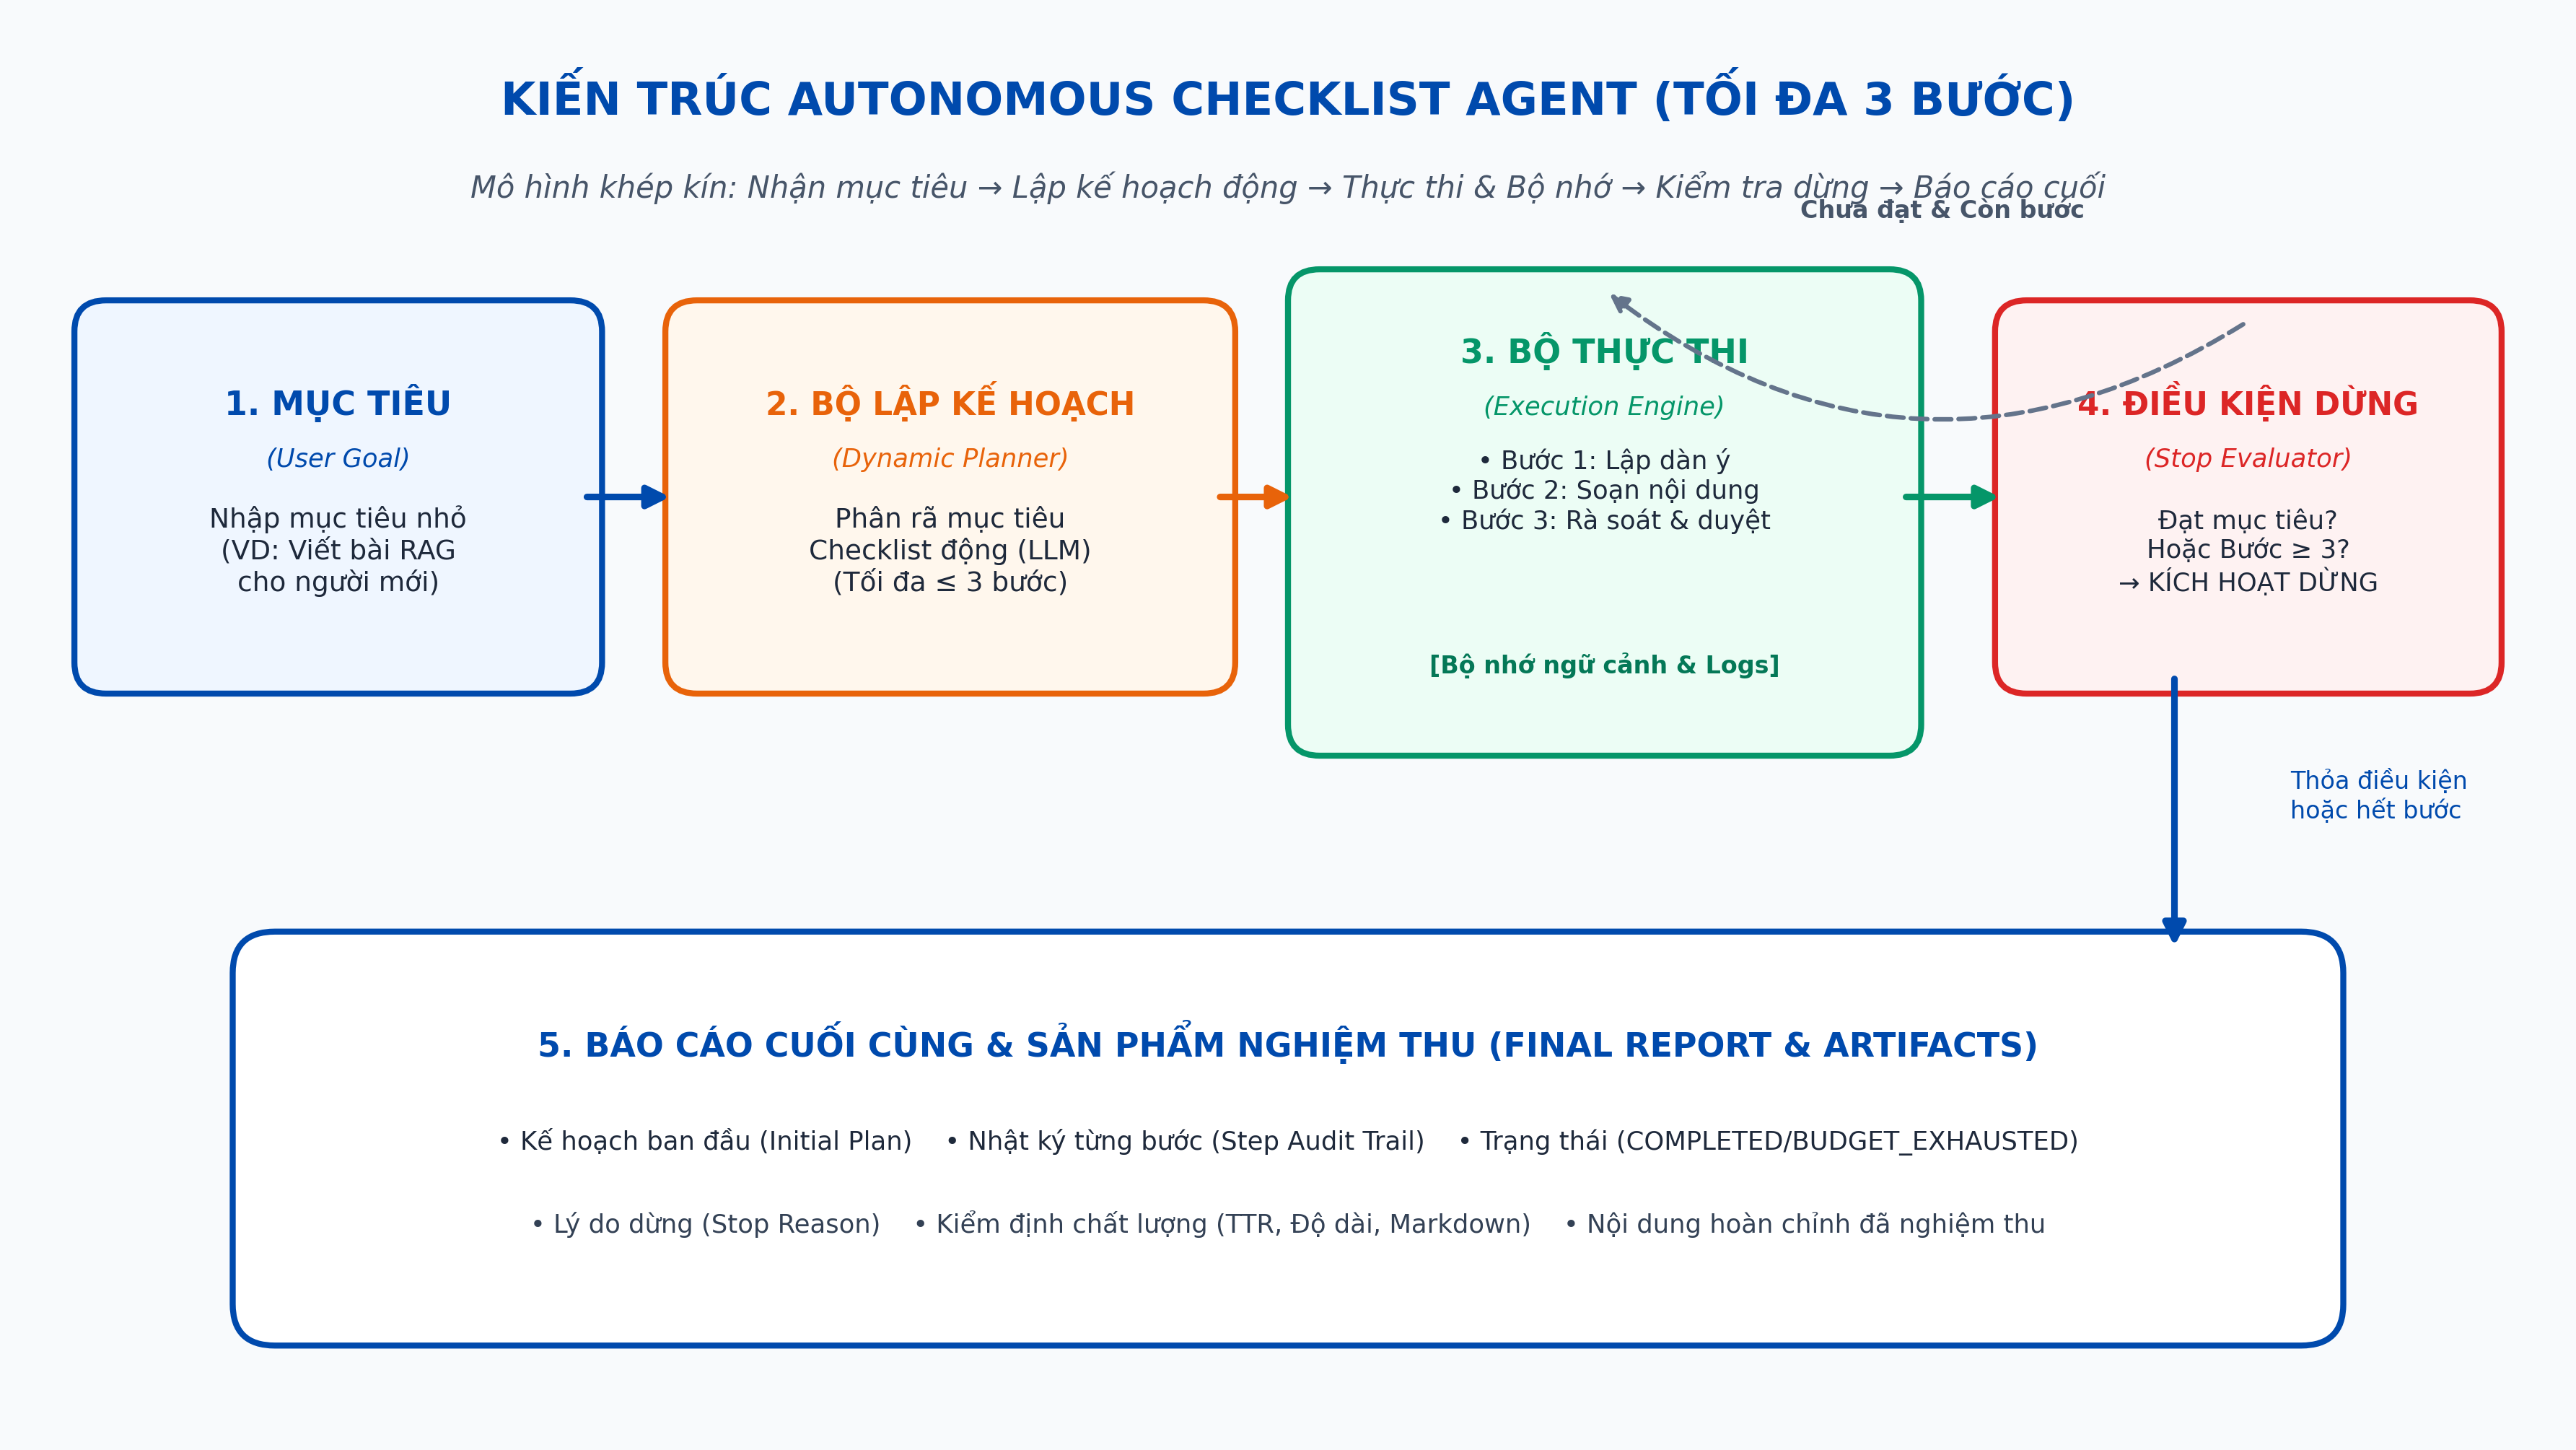
\includegraphics[width=0.95\textwidth]{images/architecture_diagram.png}
    \caption{Kiến trúc tổng thể của Autonomous Checklist Agent với vòng lặp Bounded Loop}
    \label{fig:architecture}
\end{figure}

Ngược lại, \textbf{Autonomous Agent} hoạt động dựa trên vòng lặp phản hồi khép kín (Sense - Plan - Act - Observe - Evaluate). Điểm mấu chốt tạo nên "chất tự hành" (autonomy) chính là:
\begin{enumerate}
    \item \textbf{Planner sinh kế hoạch trực tiếp từ mục tiêu:} Người dùng chỉ cung cấp Goal. Tác nhân sử dụng LLM để phân tích mục tiêu và tự sinh checklist phù hợp trong giới hạn tối đa 3 bước, thay vì chạy theo chuỗi bước viết sẵn bằng \texttt{if/elif}.
    \item \textbf{Chủ động đánh giá điều kiện dừng:} Sau mỗi bước thực thi, tác nhân tự kiểm tra xem kết quả hiện tại đã thỏa mãn mục tiêu chưa. Nếu đã đạt (\texttt{Goal Achieved}), nó chủ động ra lệnh \textbf{dừng ngay lập tức} mà không cần chạy cố các bước thừa.
\end{enumerate}

\subsection{2. Năm thành phần cốt lõi của một Checklist Agent}
Một hệ thống Autonomous Checklist Agent chuẩn mực được cấu thành từ 5 bộ phận hữu cơ:
\begin{itemize}
    \item \textbf{Tiếp nhận mục tiêu (Goal Ingestion):} Nhận câu lệnh hoặc bài toán từ người dùng (ví dụ: \textit{"Viết một bài chia sẻ ngắn giải thích RAG là gì cho người mới bắt đầu"}).
    \item \textbf{Bộ lập kế hoạch động (Dynamic Planner):} Sử dụng LLM phân tích ý định và sản sinh danh sách công việc (Checklist) với ràng buộc nghiêm ngặt: độ dài checklist không vượt quá \texttt{max\_steps} ($\le 3$ bước).
    \item \textbf{Bộ thực thi tuần tự (Sequential Executor):} Chịu trách nhiệm thực thi từng bước (sinh dàn ý, phát triển bài viết, rà soát chất lượng) dựa trên ngữ cảnh tích lũy từ các bước trước.
    \item \textbf{Bộ nhớ trạng thái ngữ cảnh (State Memory):} Đóng vai trò cầu nối dữ liệu, tích lũy kết quả của các bước trước đó để làm đầu vào cho các bước tiếp theo.
    \item \textbf{Bộ đánh giá dừng và báo cáo (Stop Evaluator \& Reporter):} Giám sát vòng lặp, kiểm soát điều kiện dừng an toàn và tổng hợp toàn bộ tiến trình thành báo cáo nghiệm thu cuối cùng.
\end{itemize}

\section{Thiết kế checklist tự động và cơ chế quản lý trạng thái}\label{thiet-ke-checklist}

\subsection{1. Kịch bản thực tế: Bài viết chia sẻ về RAG cho người mới bắt đầu}
Để chứng minh năng lực tự hành một cách thuyết phục nhất, chúng ta chọn một tác vụ cụ thể, có ranh giới rõ ràng nhưng đòi hỏi chất lượng logic cao: \textbf{"Viết một bài chia sẻ ngắn giải thích RAG là gì cho người mới bắt đầu"}. 

Thay vì hardcode cứng nhắc luôn luôn là 3 bước, tác nhân xác định checklist dựa trên mục tiêu thực tế trong giới hạn tối đa 3 bước:
\begin{itemize}
    \item \textbf{Bước 1: Xác định các ý chính cần giải thích về RAG (Action: \texttt{outline}).} Cần xác định các trọng tâm: RAG là gì, vì sao LLM cần RAG (tránh ảo giác, cập nhật dữ liệu riêng tư), cách hoạt động 3 chặng (Indexing, Retrieval, Generation), ví dụ thi mở sách dễ hiểu và lời khuyên áp dụng.
    \item \textbf{Bước 2: Viết nội dung bài chia sẻ hoàn chỉnh (Action: \texttt{generate}).} Lấy toàn bộ dàn ý từ Bước 1 làm ngữ cảnh đầu vào, phát triển thành một bài viết mạch lạc, văn phong hấp dẫn, giải thích cặn kẽ từng luận điểm.
    \item \textbf{Bước 3: Rà soát, kiểm tra độ rõ ràng và hoàn thiện (Action: \texttt{review\_polish}).} Đóng vai trò người biên tập khó tính: kiểm tra xem bài viết có quá tải thuật ngữ với người mới không, có bị lặp ý không, bổ sung lời kết và nghiệm thu chất lượng.
\end{itemize}

\textit{Lưu ý kỹ thuật về tính tự hành (Autonomy) của Planner:} Hệ thống tích hợp trực tiếp mô hình ngôn ngữ lớn (LLM Engine cục bộ qua Ollama API: \texttt{tinix-lm:latest} hoặc \texttt{qwen2.5:7b}) làm bộ não cho cả Dynamic Planner và Executor. Planner sinh kế hoạch JSON linh hoạt trực tiếp từ mục tiêu người dùng, còn Executor sinh nội dung ngữ cảnh động kèm bộ kiểm duyệt chất lượng định lượng \texttt{QualityEvaluator}. Hệ thống đồng thời tích hợp cơ chế fallback dự phòng để đảm bảo tính sẵn sàng cao khi môi trường chạy offline.

\begin{figure}[H]
    \centering
    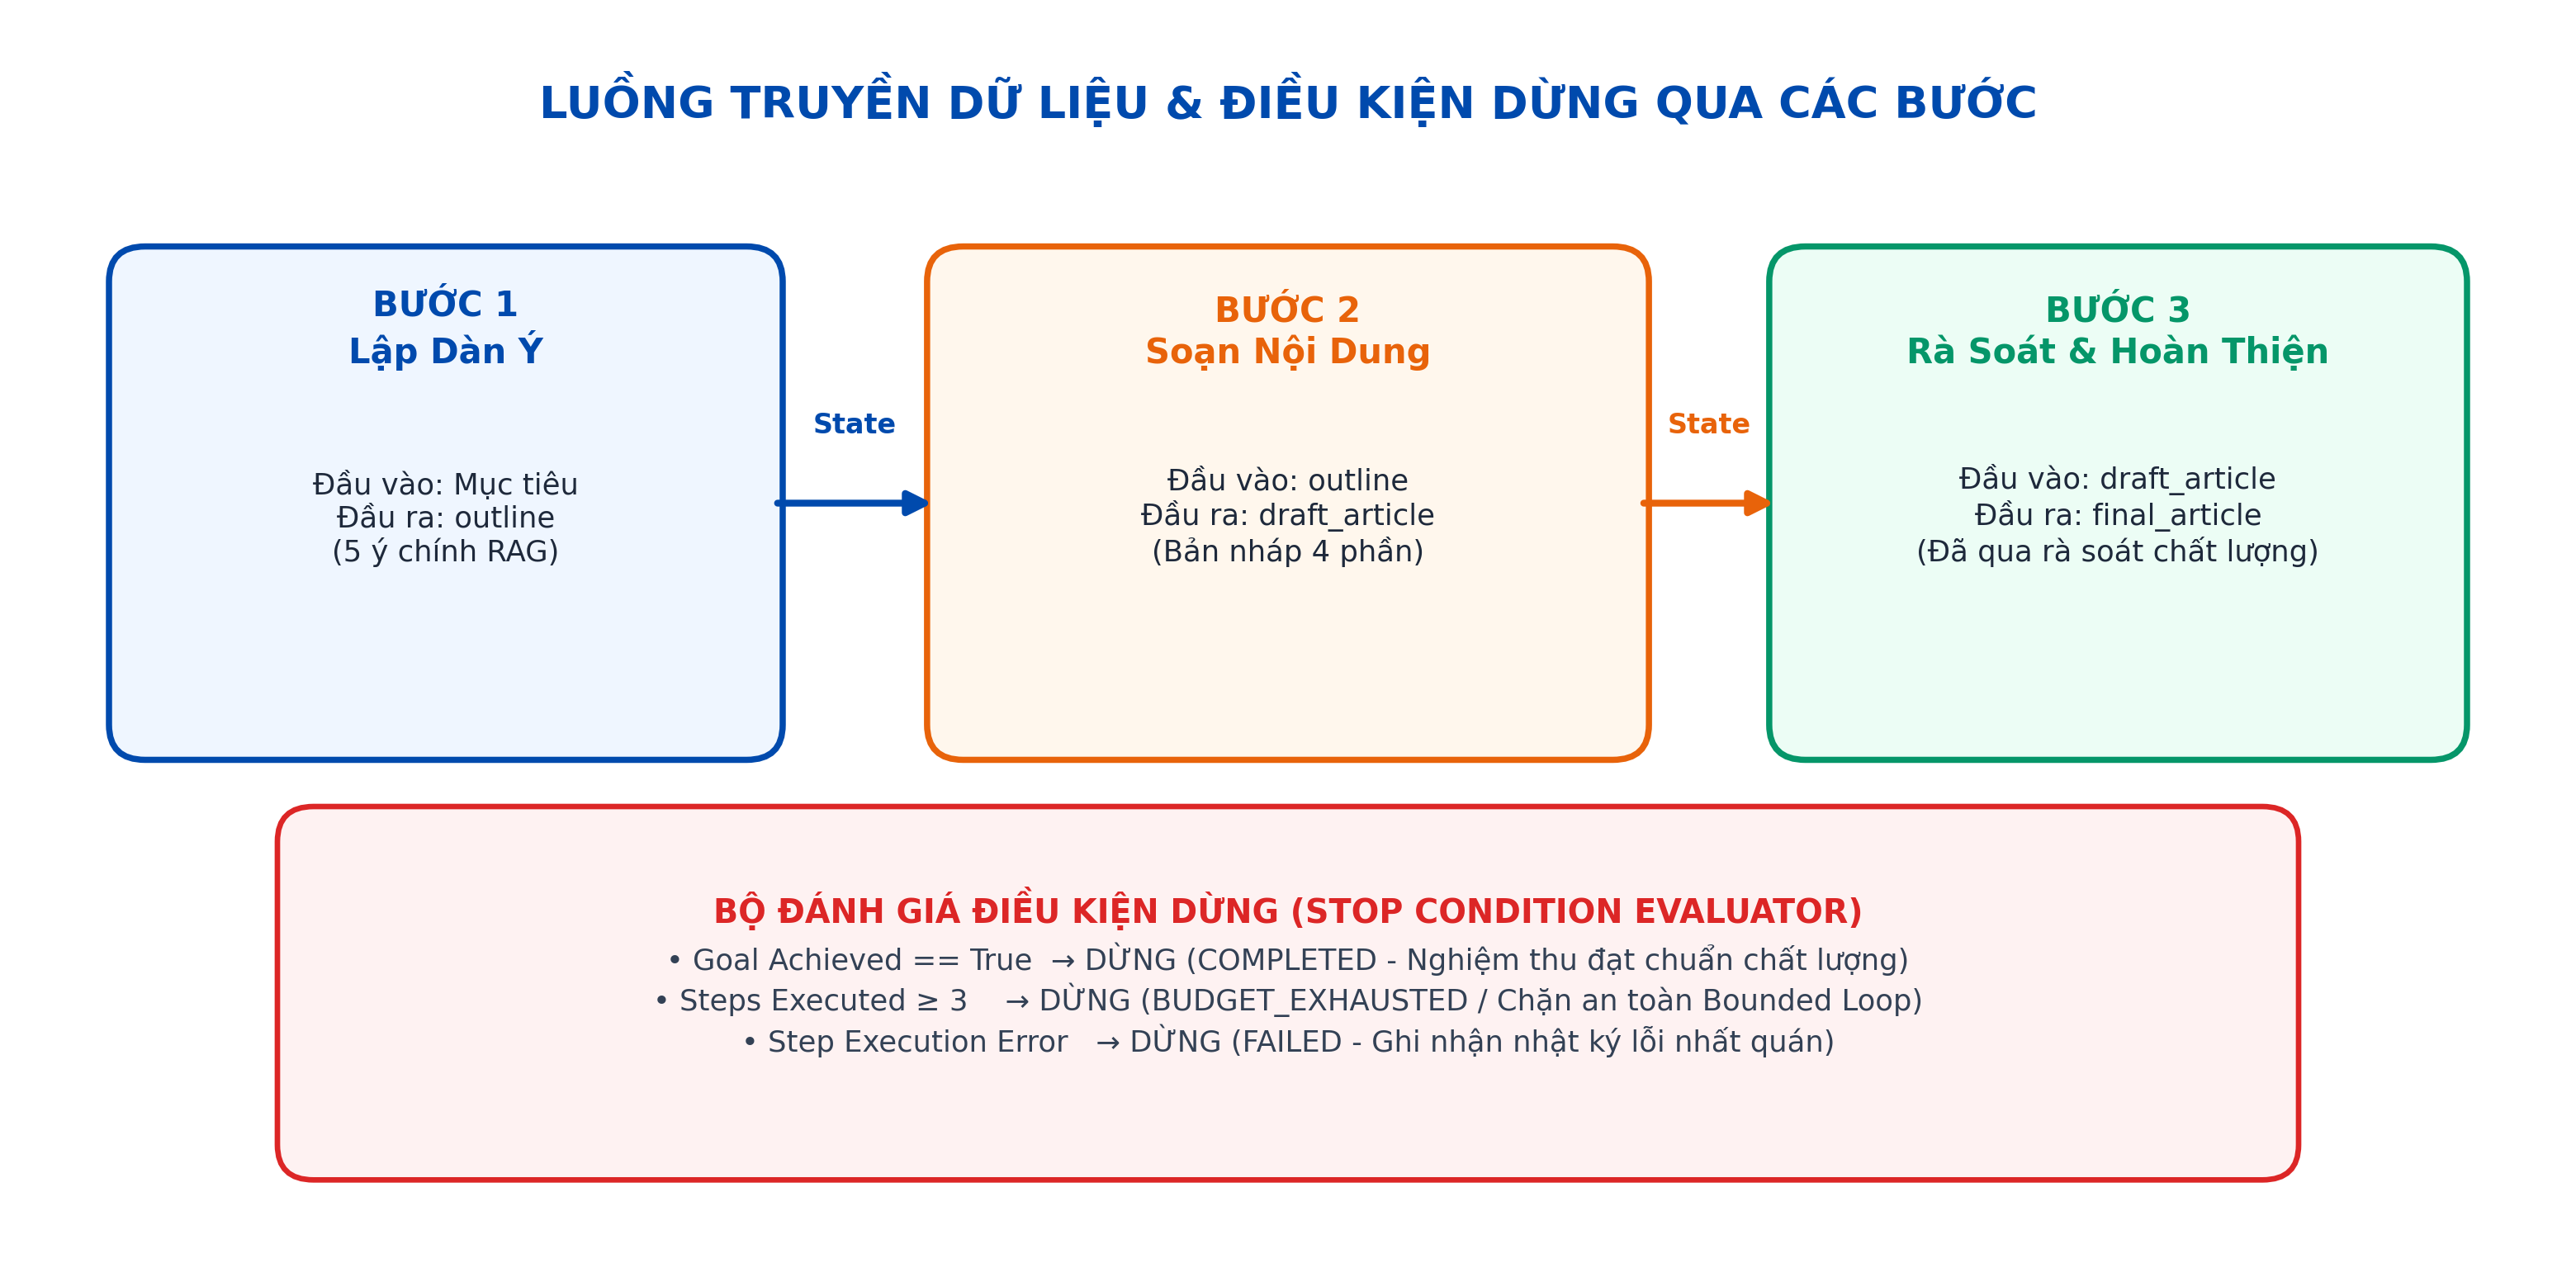
\includegraphics[width=0.9\textwidth]{images/state_flow_diagram.png}
    \caption{Luồng truyền dữ liệu qua State Memory và cơ chế rà soát điều kiện dừng ở từng bước}
    \label{fig:state_flow}
\end{figure}

\subsection{2. Cơ chế truyền trạng thái (Context Propagation)}
Như minh họa ở Hình \ref{fig:state_flow}, tính liên tục của tác nhân phụ thuộc hoàn toàn vào việc chia sẻ bộ nhớ \texttt{context\_memory}:
\begin{itemize}
    \item Khi Bước 1 kết thúc, kết quả được gắn vào khóa \texttt{context\_memory["outline"]}.
    \item Bước 2 khi bắt đầu sẽ tự động trích xuất \texttt{context\_memory["outline"]} để làm ngữ cảnh định hướng sinh bài viết, và sau khi hoàn thành sẽ lưu bản nháp vào \texttt{context\_memory["draft\_article"]}.
    \item Bước 3 trích xuất \texttt{draft\_article}, tiến hành kiểm duyệt theo bộ tiêu chí (Checklist items), bổ sung phần tổng kết và xuất ra kết quả hoàn thiện tại \texttt{context\_memory["final\_article"]}.
\end{itemize}
Nếu cơ chế truyền trạng thái này bị đứt gãy, các bước sau sẽ hoạt động "mù" (context blindness) và tác nhân sẽ không thể đạt được mục tiêu chung.

\section{Điều kiện dừng và giới hạn an toàn (Bounded Loop \& Stop Conditions)}\label{dieu-kien-dung}

\subsection{1. Hiểm họa của vòng lặp vô hạn (Infinite Loop Trap)}
Trong các hệ thống tự hành không có kiểm soát, LLM rất dễ rơi vào trạng thái "ảo giác lặp" (reasoning loop): bước sau cố gắng sửa đổi bước trước một cách không hồi kết, hoặc liên tục gọi lại cùng một công cụ với tham số tương tự. Điều này dẫn tới hai hậu quả nghiêm trọng:
\begin{enumerate}
    \item \textbf{Cạn kiệt ngân sách (Token exhaustion):} Tiêu tốn hàng nghìn USD tiền API chỉ trong vài phút.
    \item \textbf{Tắc nghẽn hệ thống (Process hanging):} Tài nguyên server bị chiếm dụng, luồng xử lý không bao giờ trả về kết quả cho người dùng.
\end{enumerate}

\subsection{2. Thiết kế Bounded Loop và bộ đánh giá dừng đa trạng thái}
Để giải quyết triệt để rủi ro trên, hệ thống của chúng ta thiết lập cơ chế kiểm soát kép phân định rõ ràng 3 trạng thái kết thúc:
\begin{enumerate}
    \item \textbf{Trạng thái hoàn thành mục tiêu (\texttt{COMPLETED}):} Sau mỗi bước, hàm \texttt{\_evaluate\_stop\_condition()} đánh giá xem sản phẩm tạo ra có thỏa mãn điều kiện nghiệm thu theo đúng mục tiêu hay không (ví dụ: mục tiêu viết bài đòi hỏi phải có \texttt{final\_article} và vượt qua kiểm định của \texttt{QualityEvaluator}). Khi thỏa mãn, hệ thống kích hoạt dừng với lý do \texttt{Goal achieved}.
    \item \textbf{Trạng thái hết ngân sách bước (\texttt{BUDGET\_EXHAUSTED}):} Khi số bước thực thi đạt ngưỡng cho phép (ví dụ \texttt{max\_steps = 1} với mục tiêu viết bài, hệ thống mới chỉ xong dàn ý), tác nhân ngắt vòng lặp an toàn và ghi nhận trạng thái \texttt{BUDGET\_EXHAUSTED} chứ không báo nhầm là \texttt{COMPLETED}.
    \item \textbf{Trạng thái thất bại (\texttt{FAILED}):} Khi một bước thực thi gặp sự cố ngoại lệ (Action failure), hệ thống ngắt phiên làm việc ngay lập tức, chuyển trạng thái sang \texttt{FAILED} và lưu vết lỗi vào Step Log.
\end{enumerate}

Nhờ đó, tác nhân vừa có tính linh hoạt tự hành, vừa tăng khả năng kiểm soát trong phạm vi các giới hạn được cấu hình.

\section{Cài đặt mã nguồn chi tiết bằng Python}\label{cai-dat-ma-nguon}

Toàn bộ hệ thống được đóng gói gọn gàng trong tệp \texttt{checklist\_agent.py} với cấu trúc hướng đối tượng rõ ràng, sử dụng triệt để thư viện tiêu chuẩn của Python để đảm bảo tính gọn nhẹ và tương thích cao nhất.

\subsection{1. Định nghĩa các cấu trúc dữ liệu cốt lõi (Data Models)}
Chúng ta sử dụng \texttt{dataclass} và \texttt{Enum} để định nghĩa kiểu dữ liệu chặt chẽ cho trạng thái, từng bước trong kế hoạch, nhật ký thực thi và báo cáo cuối cùng:

\begin{Shaded}
\begin{Highlighting}[]
\KeywordTok{class}\NormalTok{ }\DataTypeTok{AgentStatus}\NormalTok{(}\DataTypeTok{str}\NormalTok{, }\DataTypeTok{Enum}\NormalTok{):}
\NormalTok{    IDLE }\OperatorTok{=}\NormalTok{ }\StringTok{"IDLE"}
\NormalTok{    PLANNING }\OperatorTok{=}\NormalTok{ }\StringTok{"PLANNING"}
\NormalTok{    RUNNING }\OperatorTok{=}\NormalTok{ }\StringTok{"RUNNING"}
\NormalTok{    COMPLETED }\OperatorTok{=}\NormalTok{ }\StringTok{"COMPLETED"}
\NormalTok{    BUDGET_EXHAUSTED }\OperatorTok{=}\NormalTok{ }\StringTok{"BUDGET_EXHAUSTED"}
\NormalTok{    FAILED }\OperatorTok{=}\NormalTok{ }\StringTok{"FAILED"}

\AttributeTok{@dataclass}
\KeywordTok{class}\NormalTok{ }\DataTypeTok{Step}\NormalTok{:}
\NormalTok{    step_id: }\DataTypeTok{int}
\NormalTok{    title: }\DataTypeTok{str}
\NormalTok{    description: }\DataTypeTok{str}
\NormalTok{    action_type: }\DataTypeTok{str}
\NormalTok{    status: }\DataTypeTok{str} \OperatorTok{=}\NormalTok{ }\StringTok{"PENDING"}
\NormalTok{    result: }\DataTypeTok{Optional}\NormalTok{[}\DataTypeTok{str}\NormalTok{] }\OperatorTok{=}\NormalTok{ }\DataTypeTok{None}

\AttributeTok{@dataclass}
\KeywordTok{class}\NormalTok{ }\DataTypeTok{StepLog}\NormalTok{:}
\NormalTok{    step_id: }\DataTypeTok{int}
\NormalTok{    step_title: }\DataTypeTok{str}
\NormalTok{    timestamp: }\DataTypeTok{str}
\NormalTok{    duration_sec: }\DataTypeTok{float}
\NormalTok{    input_context_keys: }\DataTypeTok{List}\NormalTok{[}\DataTypeTok{str}\NormalTok{]}
\NormalTok{    output_summary: }\DataTypeTok{str}
\NormalTok{    status: }\DataTypeTok{str}
\NormalTok{    details: }\DataTypeTok{Dict}\NormalTok{[}\DataTypeTok{str}\NormalTok{, }\DataTypeTok{Any}\NormalTok{] }\OperatorTok{=}\NormalTok{ field(default_factory}\OperatorTok{=}\DataTypeTok{dict}\NormalTok{)}

\AttributeTok{@dataclass}
\KeywordTok{class}\NormalTok{ }\DataTypeTok{FinalReport}\NormalTok{:}
\NormalTok{    goal: }\DataTypeTok{str}
\NormalTok{    total_steps_planned: }\DataTypeTok{int}
\NormalTok{    steps_executed: }\DataTypeTok{int}
\NormalTok{    status: }\DataTypeTok{AgentStatus}
\NormalTok{    stop_reason: }\DataTypeTok{str}
\NormalTok{    plan: }\DataTypeTok{List}\NormalTok{[}\DataTypeTok{Dict}\NormalTok{[}\DataTypeTok{str}\NormalTok{, }\DataTypeTok{Any}\NormalTok{]]}
\NormalTok{    execution_logs: }\DataTypeTok{List}\NormalTok{[}\DataTypeTok{Dict}\NormalTok{[}\DataTypeTok{str}\NormalTok{, }\DataTypeTok{Any}\NormalTok{]]}
\NormalTok{    final_output: }\DataTypeTok{str}
\NormalTok{    quality_metrics: }\DataTypeTok{Dict}\NormalTok{[}\DataTypeTok{str}\NormalTok{, }\DataTypeTok{Any}\NormalTok{]}
\NormalTok{    total_duration_sec: }\DataTypeTok{float}
\end{Highlighting}
\end{Shaded}

\subsection{2. Bộ kiểm duyệt chất lượng định lượng (QualityEvaluator) và LLM Client}
Thay vì sử dụng các chuỗi hardcode, tác nhân tích hợp \texttt{QualityEvaluator} tính toán trực tiếp các chỉ số kỹ thuật và kết nối mô hình ngôn ngữ lớn qua \texttt{OllamaClient}:

\begin{Shaded}
\begin{Highlighting}[]
\KeywordTok{class}\NormalTok{ }\DataTypeTok{QualityEvaluator}\NormalTok{:}
    \AttributeTok{@staticmethod}
    \KeywordTok{def}\NormalTok{ }\FunctionTok{calculate_ttr}\NormalTok{(text: }\DataTypeTok{str}\NormalTok{) }\OperatorTok{->} \DataTypeTok{float}\NormalTok{:}
        \CommentTok{# Đo Type-Token Ratio (TTR): Tỷ lệ từ vựng duy nhất trên tổng số từ}
\NormalTok{        words }\OperatorTok{=}\NormalTok{ re.findall(}\StringTok{r'[a-zA-Z0-9\_]+'}\NormalTok{, text.lower())}
        \ControlFlowTok{return} \BuiltInTok{round}\NormalTok{(}\BuiltInTok{len}\NormalTok{(}\BuiltInTok{set}\NormalTok{(words)) }\OperatorTok{/} \BuiltInTok{len}\NormalTok{(words), }\DecValTok{3}\NormalTok{) }\ControlFlowTok{if}\NormalTok{ words }\ControlFlowTok{else} \FloatTok{0.0}

    \AttributeTok{@classmethod}
    \KeywordTok{def}\NormalTok{ }\FunctionTok{evaluate}\NormalTok{(}\VariableTok{cls}\NormalTok{, content: }\DataTypeTok{str}\NormalTok{, goal: }\DataTypeTok{str}\NormalTok{, intent: }\DataTypeTok{str}\NormalTok{) }\OperatorTok{->} \DataTypeTok{Dict}\NormalTok{[}\DataTypeTok{str}\NormalTok{, }\DataTypeTok{Any}\NormalTok{]:}
\NormalTok{        ttr }\OperatorTok{=} \VariableTok{cls}\NormalTok{.calculate_ttr(content)}
\NormalTok{        min_chars }\OperatorTok{=} \DecValTok{100} \ControlFlowTok{if}\NormalTok{ intent }\KeywordTok{in}\NormalTok{ (}\StringTok{"outline_only"}\NormalTok{, }\StringTok{"summarize"}\NormalTok{) }\ControlFlowTok{else} \DecValTok{250}
\NormalTok{        crit_length }\OperatorTok{=} \BuiltInTok{len}\NormalTok{(content) }\OperatorTok{>=}\NormalTok{ min_chars}
\NormalTok{        crit_structure }\OperatorTok{=} \BuiltInTok{any}\NormalTok{(line.strip().startswith((}\StringTok{'#'}\NormalTok{, }\StringTok{'-'}\NormalTok{, }\StringTok{'1.'}\NormalTok{)) }\ControlFlowTok{for}\NormalTok{ line }\KeywordTok{in}\NormalTok{ content.splitlines())}
\NormalTok{        crit_diversity }\OperatorTok{=}\NormalTok{ ttr }\OperatorTok{>=} \FloatTok{0.35}  \CommentTok{# Ngưỡng chứng minh không lặp từ}
\NormalTok{        goal_kws }\OperatorTok{=}\NormalTok{ [w }\ControlFlowTok{for}\NormalTok{ w }\KeywordTok{in}\NormalTok{ re.findall(}\StringTok{r'[a-zA-Z0-9\_]+'}\NormalTok{, goal.lower()) }\ControlFlowTok{if}\NormalTok{ len(w) }\OperatorTok{>} \DecValTok{2}\NormalTok{]}
\NormalTok{        crit_relevance }\OperatorTok{=} \BuiltInTok{any}\NormalTok{(kw }\KeywordTok{in}\NormalTok{ content.lower() }\ControlFlowTok{for}\NormalTok{ kw }\KeywordTok{in}\NormalTok{ goal_kws) }\ControlFlowTok{if}\NormalTok{ goal_kws }\ControlFlowTok{else} \ConstantTok{True}
\NormalTok{        passed }\OperatorTok{=}\NormalTok{ crit_length }\KeywordTok{and}\NormalTok{ crit_structure }\KeywordTok{and}\NormalTok{ crit_diversity }\KeywordTok{and}\NormalTok{ crit_relevance}
        \ControlFlowTok{return}\NormalTok{ \{}\StringTok{"passed"}\NormalTok{: passed, }\StringTok{"ttr"}\NormalTok{: ttr, }\StringTok{"char_count"}\NormalTok{: }\BuiltInTok{len}\NormalTok{(content)\}}
\end{Highlighting}
\end{Shaded}

\subsection{3. Lớp điều khiển tác nhân tự hành (AutonomousChecklistAgent)}
Lớp \texttt{AutonomousChecklistAgent} kết hợp LLM để tự động phân rã kế hoạch theo mục tiêu và đánh giá nghiệm thu đa trạng thái:

\begin{Shaded}
\begin{Highlighting}[]
\KeywordTok{class}\NormalTok{ }\DataTypeTok{AutonomousChecklistAgent}\NormalTok{:}
    \KeywordTok{def}\NormalTok{ }\FunctionTok{__init__}\NormalTok{(}\VariableTok{self}\NormalTok{, max_steps: }\DataTypeTok{int} \OperatorTok{=}\NormalTok{ }\DecValTok{3}\NormalTok{, use_llm: }\DataTypeTok{bool} \OperatorTok{=}\NormalTok{ }\ConstantTok{True}\NormalTok{):}
        \ControlFlowTok{if}\NormalTok{ max_steps }\OperatorTok{>}\NormalTok{ }\DecValTok{3}\NormalTok{:}
            \ControlFlowTok{raise} \DataTypeTok{ValueError}\NormalTok{(}\StringTok{f"Vi phạm Bounded Loop: max_steps (\{max_steps\}) > 3!"}\NormalTok{)}
        \VariableTok{self}\NormalTok{.max_steps }\OperatorTok{=} \BuiltInTok{min}\NormalTok{(}\BuiltInTok{max}\NormalTok{(}\DecValTok{1}\NormalTok{, max_steps), }\DecValTok{3}\NormalTok{)}
        \VariableTok{self}\NormalTok{.llm }\OperatorTok{=}\NormalTok{ OllamaClient(model}\OperatorTok{=}\StringTok{"tinix-lm:latest"}\NormalTok{) }\ControlFlowTok{if}\NormalTok{ use_llm }\ControlFlowTok{else} \ConstantTok{None}
        \VariableTok{self}\NormalTok{.evaluator }\OperatorTok{=}\NormalTok{ QualityEvaluator()}
        \VariableTok{self}\NormalTok{.context_memory }\OperatorTok{=}\NormalTok{ \{\}}

    \KeywordTok{def}\NormalTok{ }\FunctionTok{plan_steps}\NormalTok{(}\VariableTok{self}\NormalTok{, goal: }\DataTypeTok{str}\NormalTok{) }\OperatorTok{->} \DataTypeTok{List}\NormalTok{[Step]:}
        \CommentTok{# Gọi LLM sinh checklist JSON tự động theo mục tiêu hoặc qua Fallback}
        \ControlFlowTok{if} \VariableTok{self}\NormalTok{.llm }\KeywordTok{and} \VariableTok{self}\NormalTok{.llm.is_available():}
\NormalTok{            steps }\OperatorTok{=} \VariableTok{self}\NormalTok{._call_llm_planner(goal)}
            \ControlFlowTok{if}\NormalTok{ steps: }\ControlFlowTok{return}\NormalTok{ steps[:}\VariableTok{self}\NormalTok{.max_steps]}
        \ControlFlowTok{return} \VariableTok{self}\NormalTok{._heuristic_fallback_plan(goal)[:}\VariableTok{self}\NormalTok{.max_steps]}

    \KeywordTok{def}\NormalTok{ }\FunctionTok{_evaluate_stop_condition}\NormalTok{(}\VariableTok{self}\NormalTok{, idx: }\DataTypeTok{int}\NormalTok{, total: }\DataTypeTok{int}\NormalTok{, intent: }\DataTypeTok{str}\NormalTok{, goal: }\DataTypeTok{str}\NormalTok{):}
        \CommentTok{# 1. Đánh giá nghiệm thu mục tiêu (COMPLETED)}
        \ControlFlowTok{if}\NormalTok{ intent }\OperatorTok{==}\NormalTok{ }\StringTok{"outline_only"} \KeywordTok{and} \StringTok{"outline"} \KeywordTok{in} \VariableTok{self}\NormalTok{.context_memory:}
            \ControlFlowTok{if} \VariableTok{self}\NormalTok{.evaluator.evaluate(}\VariableTok{self}\NormalTok{.context_memory[}\StringTok{"outline"}\NormalTok{], goal, intent)[}\StringTok{"passed"}\NormalTok{]:}
                \ControlFlowTok{return} \ConstantTok{True}\NormalTok{, }\StringTok{"Goal achieved: Dàn ý đạt chuẩn."}\NormalTok{, AgentStatus.COMPLETED}
        \ControlFlowTok{if} \StringTok{"final_article"} \KeywordTok{in} \VariableTok{self}\NormalTok{.context_memory:}
            \ControlFlowTok{if} \VariableTok{self}\NormalTok{.evaluator.evaluate(}\VariableTok{self}\NormalTok{.context_memory[}\StringTok{"final_article"}\NormalTok{], goal, intent)[}\StringTok{"passed"}\NormalTok{]:}
                \ControlFlowTok{return} \ConstantTok{True}\NormalTok{, }\StringTok{"Goal achieved: Bài viết đạt chuẩn."}\NormalTok{, AgentStatus.COMPLETED}
        \CommentTok{# 2. Hết ngân sách bước thực thi (BUDGET_EXHAUSTED)}
        \ControlFlowTok{if}\NormalTok{ idx }\OperatorTok{>=}\NormalTok{ total:}
\NormalTok{            target_met }\OperatorTok{=}\NormalTok{ (intent }\OperatorTok{==} \StringTok{"outline_only"} \KeywordTok{and} \StringTok{"outline"} \KeywordTok{in} \VariableTok{self}\NormalTok{.context_memory) }\KeywordTok{or} \StringTok{"final_article"} \KeywordTok{in} \VariableTok{self}\NormalTok{.context_memory}
            \ControlFlowTok{if}\NormalTok{ target_met: }\ControlFlowTok{return} \ConstantTok{True}\NormalTok{, }\StringTok{"Goal achieved."}\NormalTok{, AgentStatus.COMPLETED}
            \ControlFlowTok{return} \ConstantTok{True}\NormalTok{, }\StringTok{f"Budget exhausted: Hết bước nhưng chưa đạt \{intent\}."}\NormalTok{, AgentStatus.BUDGET_EXHAUSTED}
        \ControlFlowTok{return} \ConstantTok{False}\NormalTok{, }\StringTok{"Continue"}\NormalTok{, }\ConstantTok{None}
\end{Highlighting}
\end{Shaded}

\subsection{4. Vòng lặp thực thi tự hành (Execution Loop)}
Phương thức \texttt{run()} quản trị trọn vẹn chu trình làm việc tự động khép kín kèm cơ chế bắt lỗi an toàn:

\begin{Shaded}
\begin{Highlighting}[]
    \KeywordTok{def}\NormalTok{ }\FunctionTok{run}\NormalTok{(}\VariableTok{self}\NormalTok{, goal: }\DataTypeTok{str}\NormalTok{) }\OperatorTok{->} \DataTypeTok{FinalReport}\NormalTok{:}
\NormalTok{        start_time }\OperatorTok{=}\NormalTok{ time.perf_counter()}
\NormalTok{        plan }\OperatorTok{=} \VariableTok{self}\NormalTok{.plan_steps(goal)}
\NormalTok{        topic, intent }\OperatorTok{=} \VariableTok{self}\NormalTok{._extract_topic_and_intent(goal)}
        \VariableTok{self}\NormalTok{.status }\OperatorTok{=}\NormalTok{ AgentStatus.RUNNING}

        \ControlFlowTok{for}\NormalTok{ idx, step }\KeywordTok{in} \BuiltInTok{enumerate}\NormalTok{(plan, }\DecValTok{1}\NormalTok{):}
            \ControlFlowTok{try}\NormalTok{:}
\NormalTok{                result }\OperatorTok{=} \VariableTok{self}\NormalTok{._execute_step_action(step, topic, goal)}
\NormalTok{                step.status }\OperatorTok{=}\NormalTok{ }\StringTok{"COMPLETED"}
            \ControlFlowTok{except} \DataTypeTok{Exception} \KeywordTok{as}\NormalTok{ e:}
\NormalTok{                step.status }\OperatorTok{=}\NormalTok{ }\StringTok{"FAILED"}
                \VariableTok{self}\NormalTok{.status }\OperatorTok{=}\NormalTok{ AgentStatus.FAILED}
\NormalTok{                stop_reason }\OperatorTok{=} \StringTok{f"Execution failed: Lỗi tại bước \{step.step_id\} - \{e\}"}
                \ControlFlowTok{break}

\NormalTok{            should_stop, reason, final_status }\OperatorTok{=} \VariableTok{self}\NormalTok{._evaluate_stop_condition(idx, }\BuiltInTok{len}\NormalTok{(plan), intent, goal)}
            \ControlFlowTok{if}\NormalTok{ should_stop:}
\NormalTok{                stop_reason }\OperatorTok{=}\NormalTok{ reason}
                \ControlFlowTok{if}\NormalTok{ final_status: }\VariableTok{self}\NormalTok{.status }\OperatorTok{=}\NormalTok{ final_status}
                \ControlFlowTok{break}

        \ControlFlowTok{return} \VariableTok{self}\NormalTok{._build_final_report(goal, plan, stop_reason, start_time)}
\end{Highlighting}
\end{Shaded}

\section{Thực nghiệm kịch bản: Kiểm chứng năng lực Autonomous Agent}\label{thuc-nghiem}

\subsection{1. Kịch bản 1: Viết bài chia sẻ hoàn chỉnh về RAG (3 bước đầy đủ)}
Trong kịch bản này, người dùng nhập câu lệnh mục tiêu: \textit{"Viết một bài chia sẻ ngắn giải thích RAG là gì cho người mới bắt đầu"}. Dynamic Planner nhận diện mục đích là tạo bài viết đầy đủ, từ đó sinh checklist 3 bước (Outline $\rightarrow$ Write $\rightarrow$ Review) và lần lượt thực thi như thể hiện ở Hình \ref{fig:terminal}.

\begin{figure}[H]
    \centering
    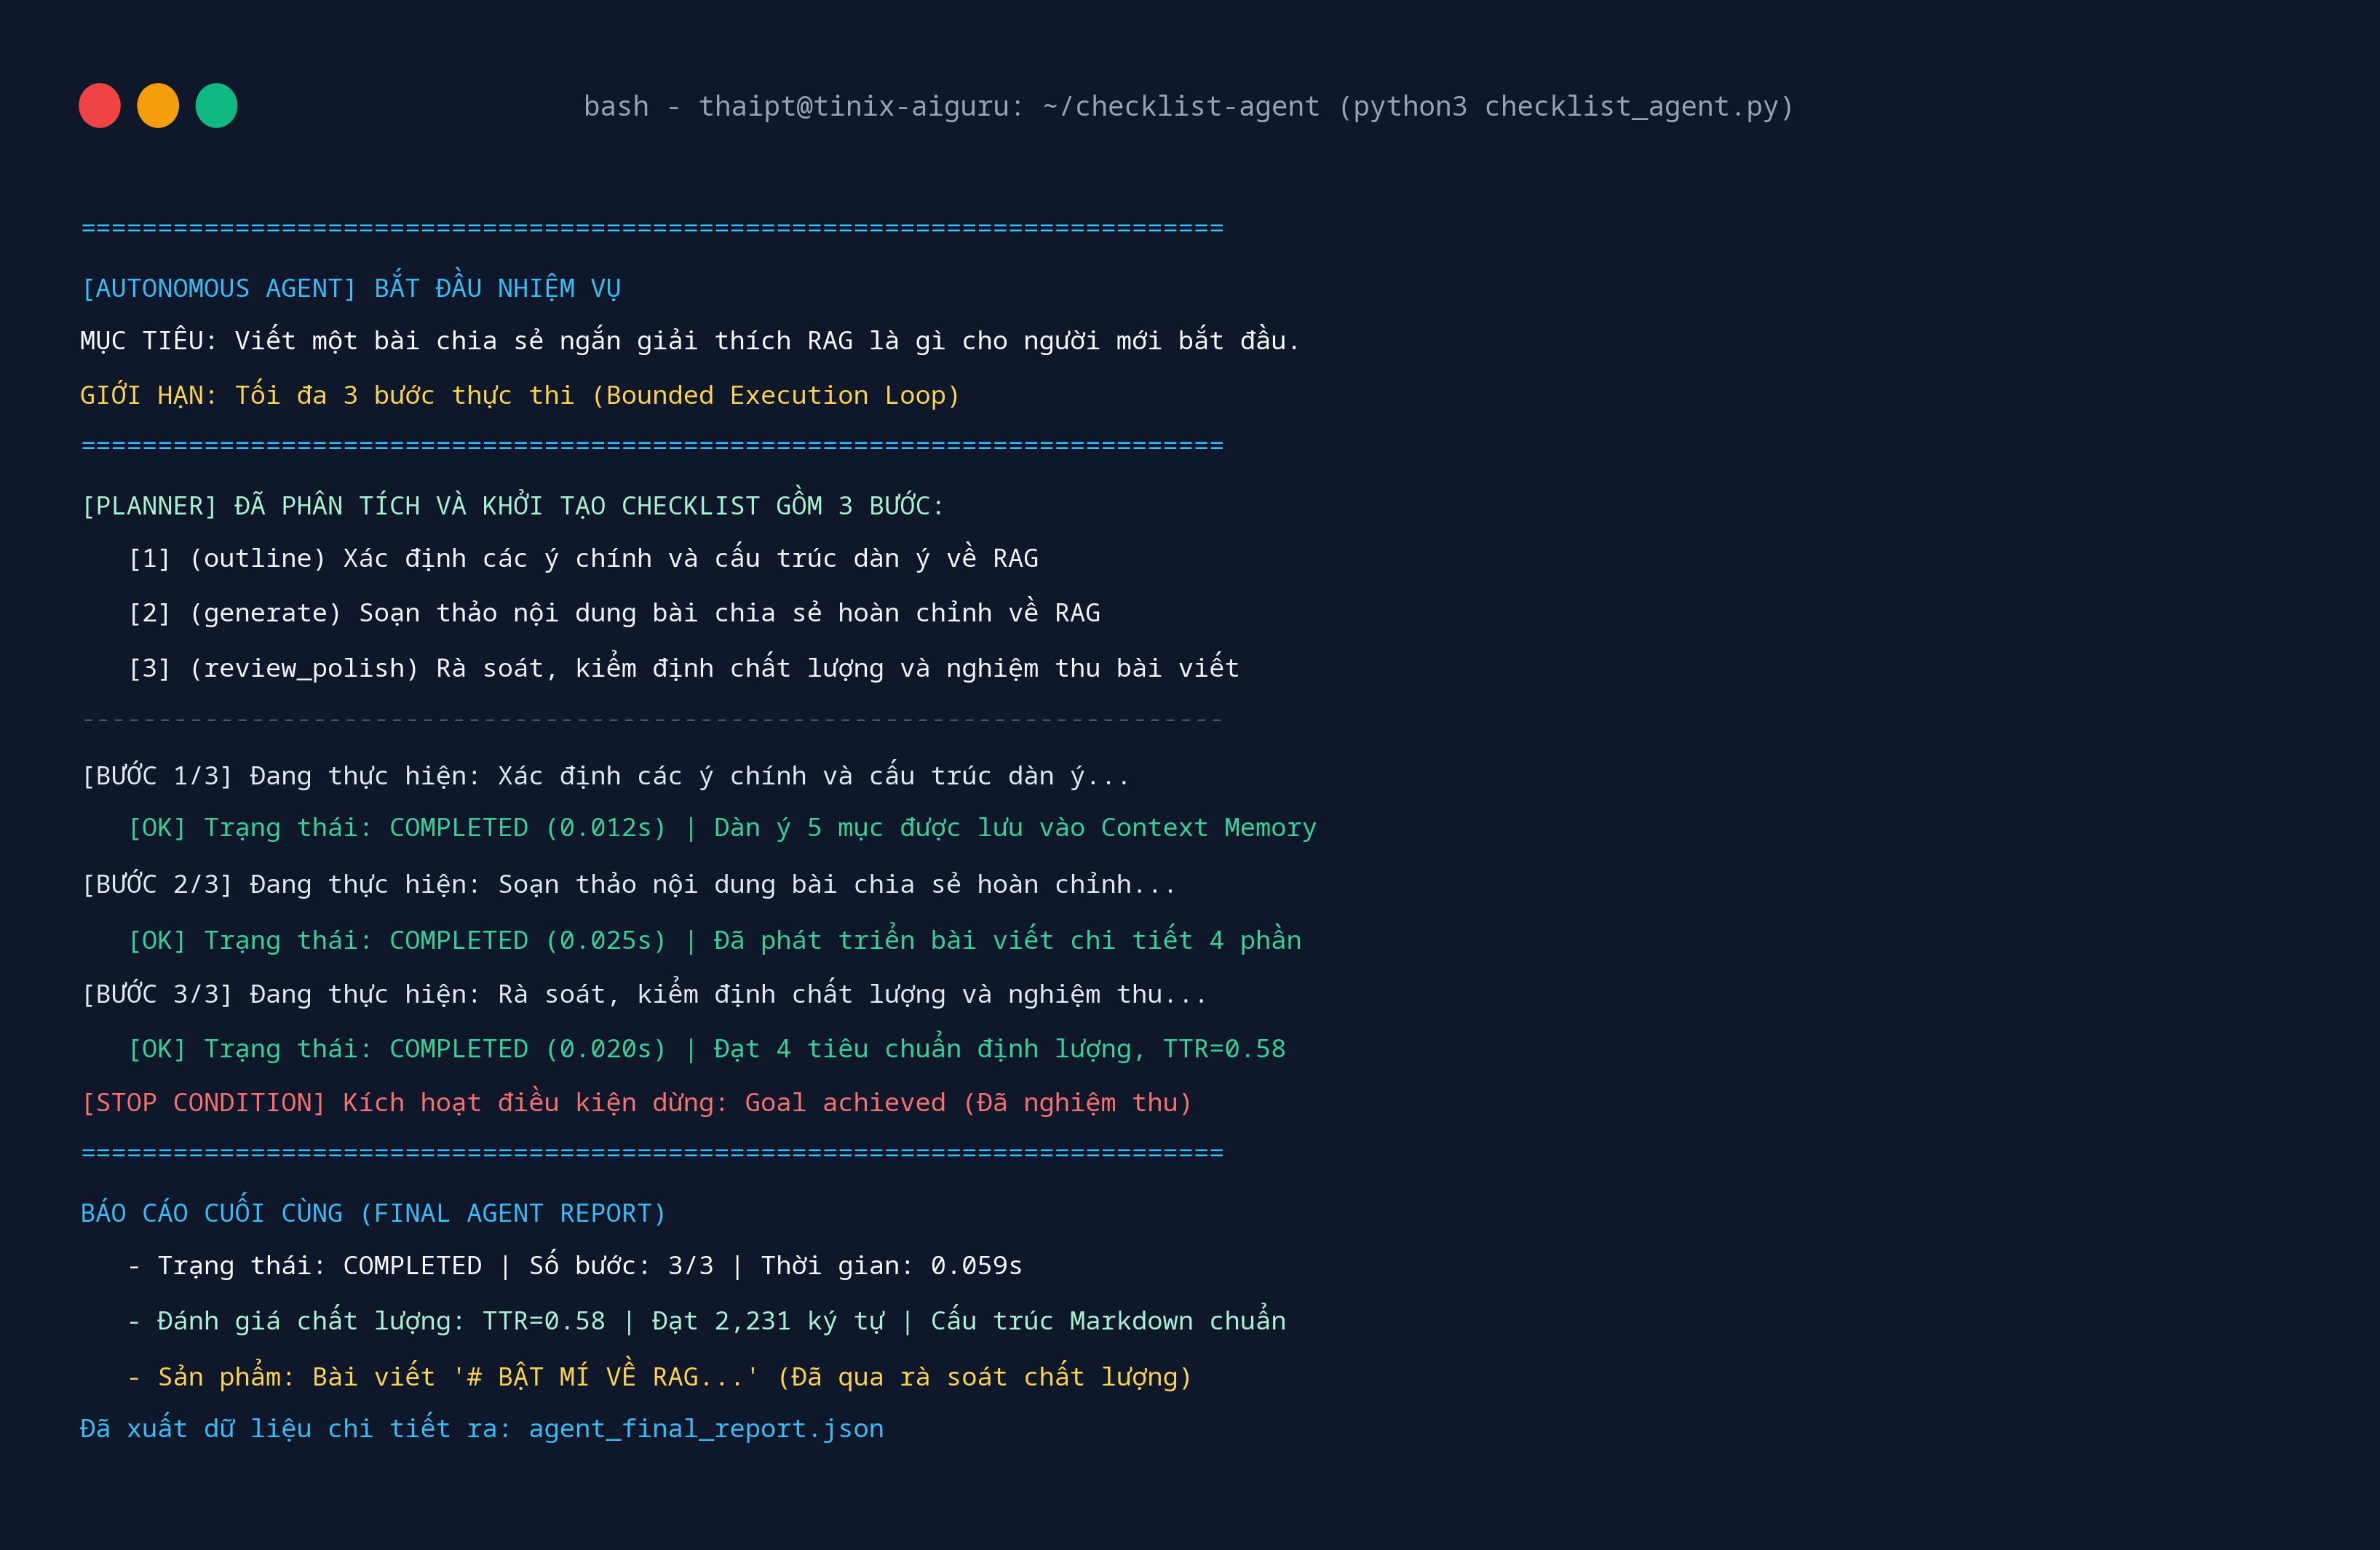
\includegraphics[width=0.78\textwidth]{images/terminal_execution.png}
    \caption{Minh họa nhật ký thực thi của Agent trên Terminal ghi nhận quá trình hoàn thành 3 bước và kích hoạt Stop Condition}
    \label{fig:terminal}
\end{figure}

Từ nhật ký thực thi minh họa, ta có thể phân tích rõ 3 chặng diễn ra:
\begin{enumerate}
    \item \textbf{Lập kế hoạch động (Dynamic Planning):} Phân tích từ khóa \textit{"RAG"} và ý định \textit{"bài chia sẻ"}, Agent tự động cấu trúc hóa danh sách 3 bước với định danh hành vi rõ ràng (\texttt{outline}, \texttt{generate}, \texttt{review\_polish}).
    \item \textbf{Thực thi và truyền dữ liệu (Context Propagation):} Bước 1 mất 0.012s tạo dàn ý; Bước 2 mất 0.025s phát triển bản nháp hoàn chỉnh; Bước 3 mất 0.020s thực hiện rà soát và chạy kiểm định chất lượng định lượng bằng \texttt{QualityEvaluator} (TTR = 0.58, độ dài 2,231 ký tự, đạt 4/4 tiêu chuẩn chất lượng).
    \item \textbf{Dừng thông minh (Stop Condition):} Sau khi hoàn thành Bước 3, bộ đánh giá nhận diện \texttt{final\_article} đã tồn tại trong \texttt{context\_memory} và kích hoạt điều kiện dừng \texttt{Goal achieved}.
\end{enumerate}

\subsection{2. Kịch bản 2: Mục tiêu nhỏ chuẩn bị Outline Docker (Tự xác định 2 bước \& Dừng sớm)}
Để minh chứng rõ nét rằng Agent \textbf{không bị hardcode cố định 3 bước}, chúng ta kiểm thử với một mục tiêu nhỏ hơn:
\begin{center}
\textit{Goal: "Chuẩn bị outline cho bài viết về Docker cho sinh viên IT."}
\end{center}
Khi nhận yêu cầu này:
\begin{itemize}
    \item \textbf{Planner thích ứng theo luật:} Tác nhân phân tích Intent/Topic theo các luật đã định nghĩa để sinh đúng số bước cần thiết (ở đây nhận thấy chỉ cần tạo dàn ý nên chỉ tạo đúng \textbf{2 bước}):
    \begin{enumerate}
        \item \textit{Bước 1 (\texttt{research\_points}):} Thu thập và xác định các luận điểm cốt lõi về Docker \& Container hóa.
        \item \textit{Bước 2 (\texttt{outline}):} Xây dựng và chuẩn hóa dàn ý chi tiết cho bài viết về Docker \& Container hóa.
    \end{enumerate}
    \item \textbf{Kích hoạt Stop Condition sớm:} Ngay khi Bước 2 hoàn thành, bộ đánh giá điều kiện dừng nhận thấy:
    \begin{center}
    \texttt{intent == "outline\_only" and "outline" in self.context\_memory}
    \end{center}
    Hệ thống lập tức kích hoạt điều kiện dừng với thông điệp: \textit{"Goal achieved: Dàn ý hoàn chỉnh đã được tạo thành công theo đúng mục tiêu."} Agent dừng ngay sau khi mục tiêu hoàn thành, tránh thực thi thêm bước không cần thiết.
\end{itemize}

Điều này minh họa khả năng thích ứng của hệ thống: không phải bài toán nào cũng ép buộc chạy hết 3 bước, mà Agent biết khi nào nhiệm vụ đã hoàn thành để chủ động dừng lại.

\subsection{3. So sánh chất lượng sản phẩm giữa các bước}
Bảng \ref{tab:so-sanh-chat-luong} đối chiếu sự tiến hóa rõ rệt về chất lượng nội dung giữa bản nháp sau Bước 2 và bản hoàn thiện sau Bước 3 nhờ cơ chế Context Propagation:

\renewcommand{\arraystretch}{1.3}
\begin{longtable}{|p{0.45\textwidth}|p{0.48\textwidth}|}
\caption{Đối chiếu chất lượng nội dung qua chuỗi truyền trạng thái} \label{tab:so-sanh-chat-luong} \\
\hline
\rowcolor{primary!15}
\textbf{Bản nháp sau Bước 2 (Soạn thảo thô)} & \textbf{Bản hoàn thiện sau Bước 3 (Đã rà soát)} \\ \hline
\endfirsthead
\hline
\rowcolor{primary!15}
\textbf{Bản nháp sau Bước 2 (Soạn thảo thô)} & \textbf{Bản hoàn thiện sau Bước 3 (Đã rà soát)} \\ \hline
\endhead
Đã có định nghĩa cơ bản và 3 chặng Indexing $\rightarrow$ Retrieval $\rightarrow$ Generation. & Bổ sung thêm ví dụ so sánh đời thường: học sinh thi "mở sách" vs "đóng sách" giúp người mới dễ hiểu ngay lập tức. \strut \tabularnewline \hline
Kết thúc đột ngột ở phần mô tả kỹ thuật, người đọc chưa biết bước tiếp theo nên bắt đầu từ đâu. & Bổ sung mục Lời kết thực tế: hướng dẫn người mới bắt đầu với thư viện mã nguồn mở (ChromaDB, Qdrant kết hợp LangChain).\strut \tabularnewline \hline
\raggedright Chưa được kiểm chứng tính nhất quán về thuật ngữ.\strut & \raggedright Đã qua kiểm định định lượng bằng \texttt{QualityEvaluator}: TTR = 0.58 (ngưỡng $\ge 0.35$ chứng minh không trùng lặp từ), độ dài 2,231 ký tự, chuẩn hóa cấu trúc Markdown phân cấp.\strut \tabularnewline \hline
\hline
\end{longtable}
\renewcommand{\arraystretch}{1.0}


\subsection{4. Kiểm thử toàn diện 7 kịch bản biên và xử lý lỗi (Comprehensive Test Suite)}
Nhằm đảm bảo hệ thống phản ứng nhất quán và chính xác trước mọi tình huống thực tế (bao gồm các ca biên và sự cố), bộ kiểm thử \texttt{eval\_agent.py} được thiết kế với 7 kịch bản kiểm tra nghiêm ngặt:

\renewcommand{\arraystretch}{1.05}
\begin{longtable}{|p{0.05\textwidth}|p{0.34\textwidth}|p{0.21\textwidth}|p{0.28\textwidth}|}
\caption{Kết quả kiểm thử 7 kịch bản đánh giá năng lực tác nhân tự hành} \label{tab:test-cases} \\
\hline
\rowcolor{primary!15}
\textbf{STT} & \textbf{Kịch bản kiểm thử (Test Scenario)} & \textbf{Trạng thái} & \textbf{Điều kiện dừng / Kết quả} \\ \hline
\endfirsthead
\hline
\rowcolor{primary!15}
\textbf{STT} & \textbf{Kịch bản kiểm thử (Test Scenario)} & \textbf{Trạng thái} & \textbf{Điều kiện dừng / Kết quả} \\ \hline
\endhead
1 & Viết bài RAG hoàn chỉnh (3 bước) & \texttt{COMPLETED} & \texttt{Goal achieved} (Đạt 4 tiêu chuẩn) \\ \hline
2 & Chuẩn bị outline Docker (2 bước) & \texttt{COMPLETED} & \texttt{Goal achieved} (Dừng sớm an toàn) \\ \hline
3 & Tóm tắt tài liệu MCP (2 bước) & \texttt{COMPLETED} & \texttt{Goal achieved} (Bản tóm tắt súc tích) \\ \hline
4 & Hết bước chưa đạt mục tiêu (\texttt{max\_steps=1} viết bài) & \texttt{BUDGET\_EXHAUSTED} & \texttt{Budget exhausted} (Không báo nhầm COMPLETED) \\ \hline
5 & Mục tiêu mở tùy ý (Tối ưu PostgreSQL) & \texttt{COMPLETED} & \texttt{Goal achieved} (Thích ứng linh hoạt) \\ \hline
6 & Sự cố thực thi (Action Exception) & \texttt{FAILED} & \texttt{Execution failed} (Ghi log lỗi) \\ \hline
7 & Rào chắn an toàn Bounded Loop (\texttt{max\_steps=5}) & \texttt{PASSED} & Chặn đứng vi phạm (\texttt{ValueError}) \\ \hline
\hline
\end{longtable}
\renewcommand{\arraystretch}{1.0}

\section{Phân tích Báo cáo Cuối Cùng (Final Report) và Nhật ký Bước (Step Logs)}\label{phan-tich-bao-cao}

Sau khi kết thúc phiên làm việc, Agent tự động kết xuất tệp tin \texttt{agent\_final\_report.json}. Dưới đây là cấu trúc tệp tin kiểm toán thực tế được sinh ra:

\begin{Shaded}
\begin{Highlighting}[]
\NormalTok{\{}
\NormalTok{  }\DataTypeTok{"goal"}\NormalTok{: }\StringTok{"Viết một bài chia sẻ ngắn giải thích RAG là gì cho người mới bắt đầu."}\NormalTok{,}
\NormalTok{  }\DataTypeTok{"total_steps_planned"}\NormalTok{: }\DecValTok{3}\NormalTok{,}
\NormalTok{  }\DataTypeTok{"steps_executed"}\NormalTok{: }\DecValTok{3}\NormalTok{,}
\NormalTok{  }\DataTypeTok{"status"}\NormalTok{: }\StringTok{"COMPLETED"}\NormalTok{,}
\NormalTok{  }\DataTypeTok{"stop_reason"}\NormalTok{: }\StringTok{"Goal achieved: Bài viết đã được tạo và rà soát hoàn tất theo đúng mục tiêu."}\NormalTok{,}
\NormalTok{  }\DataTypeTok{"plan"}\NormalTok{: [}
\NormalTok{    \{}\DataTypeTok{"step_id"}\NormalTok{: }\DecValTok{1}\NormalTok{, }\DataTypeTok{"title"}\NormalTok{: }\StringTok{"Xác định các ý chính cần giải thích về RAG"}\NormalTok{, }\DataTypeTok{"status"}\NormalTok{: }\StringTok{"COMPLETED"}\NormalTok{\},}
\NormalTok{    \{}\DataTypeTok{"step_id"}\NormalTok{: }\DecValTok{2}\NormalTok{, }\DataTypeTok{"title"}\NormalTok{: }\StringTok{"Viết nội dung bài chia sẻ hoàn chỉnh"}\NormalTok{, }\DataTypeTok{"status"}\NormalTok{: }\StringTok{"COMPLETED"}\NormalTok{\},}
\NormalTok{    \{}\DataTypeTok{"step_id"}\NormalTok{: }\DecValTok{3}\NormalTok{, }\DataTypeTok{"title"}\NormalTok{: }\StringTok{"Rà soát, kiểm tra độ rõ ràng và hoàn thiện bài viết"}\NormalTok{, }\DataTypeTok{"status"}\NormalTok{: }\StringTok{"COMPLETED"}\NormalTok{\}}
\NormalTok{  ],}
\NormalTok{  }\DataTypeTok{"execution_logs"}\NormalTok{: [}
\NormalTok{    \{}\DataTypeTok{"step_id"}\NormalTok{: }\DecValTok{1}\NormalTok{, }\DataTypeTok{"duration_sec"}\NormalTok{: }\FloatTok{0.012}\NormalTok{, }\DataTypeTok{"input_context_keys"}\NormalTok{: [], }\DataTypeTok{"status"}\NormalTok{: }\StringTok{"COMPLETED"}\NormalTok{,}
\NormalTok{     }\DataTypeTok{"output_summary"}\NormalTok{: }\StringTok{"DÀN Ý BÀI VIẾT: TÌM HIỂU RAG CHO NGƯỜI MỚI BẮT ĐẦU..."}\NormalTok{\},}
\NormalTok{    \{}\DataTypeTok{"step_id"}\NormalTok{: }\DecValTok{2}\NormalTok{, }\DataTypeTok{"duration_sec"}\NormalTok{: }\FloatTok{0.025}\NormalTok{, }\DataTypeTok{"input_context_keys"}\NormalTok{: [}\StringTok{"outline"}\NormalTok{], }\DataTypeTok{"status"}\NormalTok{: }\StringTok{"COMPLETED"}\NormalTok{,}
\NormalTok{     }\DataTypeTok{"output_summary"}\NormalTok{: }\StringTok{"# BẬT MÍ VỀ RAG: 'VŨ KHÍ TỐI THƯỢNG' GIÚP AI THÔNG MINH..."}\NormalTok{\},}
\NormalTok{    \{}\DataTypeTok{"step_id"}\NormalTok{: }\DecValTok{3}\NormalTok{, }\DataTypeTok{"duration_sec"}\NormalTok{: }\FloatTok{0.018}\NormalTok{, }\DataTypeTok{"input_context_keys"}\NormalTok{: [}\StringTok{"outline"}\NormalTok{, }\StringTok{"draft_article"}\NormalTok{], }\DataTypeTok{"status"}\NormalTok{: }\StringTok{"COMPLETED"}\NormalTok{,}
\NormalTok{     }\DataTypeTok{"output_summary"}\NormalTok{: }\StringTok{"# BẬT MÍ VỀ RAG: 'VŨ KHÍ TỐI THƯỢNG' GIÚP AI THÔNG MINH..."}\NormalTok{\}}
\NormalTok{  ],}
\NormalTok{  }\DataTypeTok{"total_duration_sec"}\NormalTok{: }\FloatTok{0.056}
\NormalTok{\}}
\end{Highlighting}
\end{Shaded}

Báo cáo này mang lại giá trị cốt lõi về mặt kỹ thuật:
\begin{itemize}
    \tightlist
    \item \textbf{Tính minh bạch (Observability):} Bất kỳ ai kiểm tra hệ thống cũng thấy rõ từng bước chạy mất bao lâu, tiêu thụ những khóa ngữ cảnh nào (\texttt{input\_context\_keys}) và cho ra kết quả gì.
    \item \textbf{Khả năng tái lập (Reproducibility):} Giúp kỹ sư dễ dàng truy vết xem lỗi phát sinh từ khâu lập kế hoạch (Planner) hay khâu thực thi (Executor).
\end{itemize}

\section{Mở rộng và Ứng dụng thực tế của Checklist Agent}\label{mo-rong-ung-dung}

Mô hình Checklist Agent 3 bước có thể mở rộng linh hoạt cho rất nhiều bài toán sản xuất thực tế tại doanh nghiệp:

\textbf{1. Trợ lý Tự động Viết Tài liệu API (Technical Documentation Agent):}
Khi một lập trình viên hoàn thành một endpoint mới, họ chỉ cần đưa mã nguồn vào với mục tiêu: \textit{"Viết tài liệu Swagger/Markdown cho API thanh toán"}. Agent tự phân rã:
\begin{itemize}
    \tightlist
    \item \textit{Bước 1:} Quét hàm để bóc tách tham số đầu vào/đầu ra và các mã lỗi (Error codes).
    \item \textit{Bước 2:} Sinh tài liệu chi tiết kèm ví dụ cURL.
    \item \textit{Bước 3:} Rà soát cú pháp chuẩn OpenAPI Spec $\rightarrow$ Nghiệm thu $\rightarrow$ Lưu file.
\end{itemize}

\textbf{2. Trợ lý Rà soát Pull Request (PR Code Reviewer Agent):}
Với mục tiêu: \textit{"Kiểm tra bảo mật và chuẩn coding style cho PR \#104"}:
\begin{itemize}
    \tightlist
    \item \textit{Bước 1:} Trích xuất \texttt{git diff} những file thay đổi.
    \item \textit{Bước 2:} Đối chiếu với bộ quy tắc an ninh (kiểm tra rò rỉ secret, SQL injection, null check).
    \item \textit{Bước 3:} Tổng hợp comment góp ý và gửi thông báo lên GitHub/GitLab.
\end{itemize}

\textbf{3. Trợ lý Tự động Hóa Chăm sóc Khách hàng Cấp cao:}
Nhận khiếu nại phức tạp từ khách hàng, Agent tự chia bước:
\begin{itemize}
    \tightlist
    \item \textit{Bước 1:} Tra cứu lịch sử đơn hàng trong cơ sở dữ liệu nội bộ.
    \item \textit{Bước 2:} Đối chiếu với chính sách đổi trả hiện hành của công ty.
    \item \textit{Bước 3:} Soạn email phản hồi thấu cảm, đưa ra phương án bồi hoàn và lưu log vào hệ thống CRM.
\end{itemize}

\section{Kết luận}\label{ket-luan}

Xây dựng hệ thống tác nhân tự hành (\textbf{Autonomous Systems}) không đòi hỏi những mô hình ma thuật phức tạp, mà bắt đầu từ những nguyên lý kỹ thuật vững chắc: \textbf{Mục tiêu rõ ràng $\rightarrow$ Lập kế hoạch có cấu trúc $\rightarrow$ Thực thi tuần tự có quản lý trạng thái $\rightarrow$ Giới hạn số bước an toàn $\rightarrow$ Điều kiện dừng chuẩn xác}.

Thông qua bài học này, bạn đã tự tay thiết kế và vận hành thành công một Autonomous Checklist Agent giải quyết bài toán viết bài chia sẻ RAG cho người mới bắt đầu. Mô hình khép kín này là nền tảng tối quan trọng giúp bạn tự tin bước vào những bài toán phức tạp hơn như Multi-Agent Systems, Hierarchical Planning và Graph-based Autonomous Workflows trong tương lai.

\textbf{Mã nguồn đầy đủ và Kịch bản kiểm thử (Repository):}\\
Toàn bộ mã nguồn \texttt{checklist\_agent.py}, bộ kiểm thử \texttt{eval\_agent.py}, script sinh ảnh \texttt{generate\_assets.py} cùng báo cáo \texttt{agent\_final\_report.json} được lưu trữ công khai tại GitHub: \\
\url{https://github.com/thaiptit123/autonomous-checklist-agent}

\section{Tài liệu tham khảo}\label{tai-lieu-tham-khao}

\begin{enumerate}
    \tightlist
    \def\labelenumi{[\arabic{enumi}]}
    \item \textbf{Anthropic}: \textit{Building Effective Agents}. Bài viết kinh điển phân tích ranh giới giữa Workflow và Autonomous Agent. \url{https://www.anthropic.com/research/building-effective-agents}
    \item \textbf{LangChain / LangGraph Documentation}: Khung phát triển ứng dụng tác nhân có trạng thái và vòng lặp kiểm soát. \url{https://langchain-ai.github.io/langgraph/}
    \item \textbf{Lewis et al.}: \textit{Retrieval-Augmented Generation for Knowledge-Intensive NLP Tasks}. Nghiên cứu gốc giới thiệu kỹ thuật RAG. \url{https://arxiv.org/abs/2005.11401}
    \item \textbf{ReAct Framework}: \textit{Synergizing Reasoning and Acting in Language Models} (Yao et al., ICLR 2023). \url{https://arxiv.org/abs/2210.03629}
    \item \textbf{AI Guru x TiniX Tutorial Series}: Chuỗi tài liệu chuẩn định dạng nội bộ cho các khóa đào tạo kỹ sư AI.
\end{enumerate}

\end{document}
